\documentclass{standalone}
\usepackage{tikz}
\usetikzlibrary{arrows.meta}
\tikzset{>={Latex[width=3mm,length=3mm]}}
\usepackage {xcolor}
\usepackage{pgf}
\usepackage{pgfplots}
\usetikzlibrary{decorations}

\begin{document}

\scalebox{0.8}{
	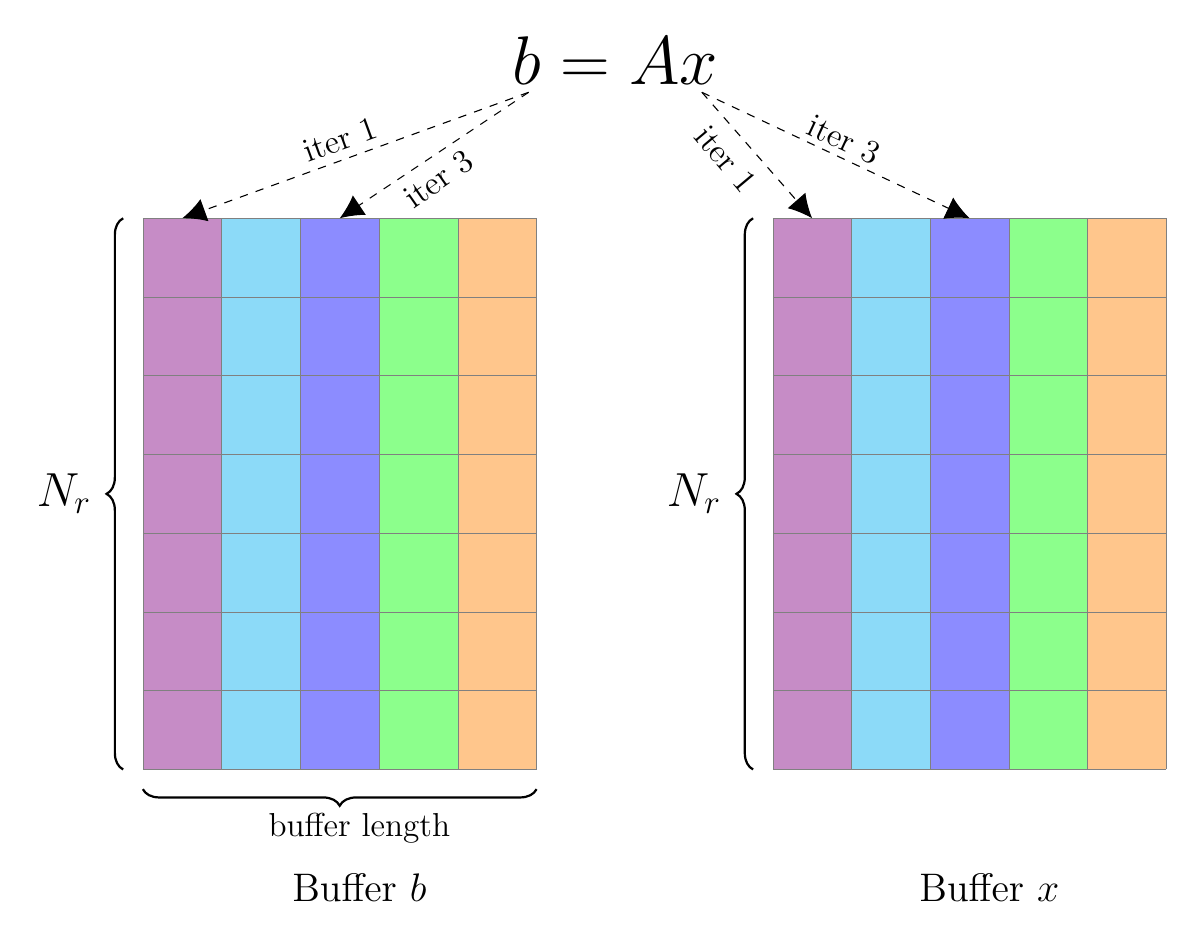
\begin{tikzpicture}[decoration={brace,amplitude=6pt}]
	\fill[violet!45!white] (-1,-2) rectangle (0,5); 
	\fill[cyan!45!white] (0,-2) rectangle (1,5); 
	\fill[blue!45!white] (1,-2) rectangle (2,5); 
	\fill[green!45!white] (2,-2) rectangle (3,5); 
	\fill[orange!45!white] (3,-2) rectangle (4,5); 
%	\fill[green!55!white] (4,-3) rectangle (5,7); 
%	\fill[yellow!45!white] (5,-3) rectangle (6,7); 
%	\fill[] (6,-3) rectangle (7,7); 
%	\fill[red!45!white] (7,-3) rectangle (8,7); 

	
	\draw[step=1cm,gray,very thin] (-1,-2) grid (4,5);

	\draw[thick] [decorate,color=black] (-1.25,-2) -- (-1.25,5);
	\node at (-2,1.5) {\LARGE{$N_r$}};
	\draw[thick] [decorate,color=black]  (4,-2.25) -- (-1,-2.25);
	\node at (1.75,-2.75)  {\large{buffer length}};
%	\node at 

\begin{scope}[shift={(8,0)}]
	\fill[violet!45!white] (-1,-2) rectangle (0,5); 
	\fill[cyan!45!white] (0,-2) rectangle (1,5); 
	\fill[blue!45!white] (1,-2) rectangle (2,5); 
	\fill[green!45!white] (2,-2) rectangle (3,5); 
	\fill[orange!45!white] (3,-2) rectangle (4,5); 
	%	\fill[green!55!white] (4,-3) rectangle (5,7); 
	%	\fill[yellow!45!white] (5,-3) rectangle (6,7); 
	%	\fill[] (6,-3) rectangle (7,7); 
	%	\fill[red!45!white] (7,-3) rectangle (8,7); 
	
	
	\draw[step=1cm,gray,very thin] (-1,-2) grid (4,5);
	
	\draw[thick] [decorate,color=black] (-1.25,-2) -- (-1.25,5);
	\node at (-2,1.5) {\LARGE{$N_r$}};
%	\draw[thick] [decorate,color=black]  (4,-3.25) -- (-1,-3.25);
%	\node at (1.75,-3.75)  {\large{buffer length}};
\end{scope}
\node at (5,7) {\Huge{$b=A x$}};

%iter 1
\draw[->,dashed] (3.9,6.6) -- (-0.5,5);
\draw[->,dashed] (6.1,6.6) -- (7.5,5);
\node[rotate=20] at (1.5,6) {\large{iter 1}};
\node[rotate=35] at (2.75,5.5) {\large{iter 3}};

%iter 2
\draw[->,dashed] (3.9,6.6) -- (1.5,5);
\draw[->,dashed] (6.1,6.6) -- (9.5,5);
\node[rotate=-50] at (6.4,5.75) {\large{iter 1}};
\node[rotate=-25] at (7.9,6) {\large{iter 3}};
\node at (1.75, -3.5) {\Large{Buffer $b$}};
\node at (9.75, -3.5) {\Large{Buffer $x$}};
	\end{tikzpicture}
}

\end{document}
